\documentclass[a4paper,12pt]{article}
\usepackage[margin=1in]{geometry}

\usepackage[T2A]{fontenc}			% кодировка
\usepackage[utf8]{inputenc}			% кодировка исходного текста
\usepackage[english,russian]{babel}	% локализация и переносы
\usepackage{graphicx}                % Математика
\usepackage{amsmath,amsfonts,amssymb,amsthm,mathtools} 
\usepackage{mathtext}
\usepackage[T2A]{fontenc}
\usepackage[utf8]{inputenc}

\usepackage{wasysym}

%Заговолок
\author{Бичина Марина 
группа Б04-005 1 курса ФЭФМ}
\title{}
\date{}


\begin{document} % начало документа

\begin{center}
\begin{Large}
{Корнеев Николай Б04-005, Лабораторная работа №. 4.7.3 <<Поляризация>>}
\end{Large}
\end{center}
\paragraph{Цель работы:} 
ознакомиться с методами получения и анализа поляризованного света
\begin{enumerate}
\itemsep0em
\item oпределить разрешенные направления поляроидов
\item определить характер поляризации света, прошедшего стопу и отраженного от нее под углом Брюстера
\item оценить угол Брюстера для эбонита
\item выделить пластинки $\lambda/2$ и $\lambda/4$
\item определить направления большей и меньшей скоростей для пластинки $\lambda/4$
\item исследовать интерференцию поляризованных лучей
\end{enumerate}
\paragraph{Оборудование:}
\begin{enumerate}
\itemsep0em
\item оптическая скамья с осветителем
\item зеленый светофильтр
\item два поляроида
\item черное зеркало
\item полированная эбонитовая пластинка
\item стопа стеклянных пластинок
\item слюдяные пластинки разной толщины
\item пластинки $\lambda/2$ и $\lambda/4$
\item пластинка в одну длину волны для зеленого света
\end{enumerate}


\paragraph{Теоретическая справка:}
При помощи поляризаторов, естественный свет может быть превращен в линейно поляризованный, для которого характерно то, что пара векторов \textbf{E} и \textbf{H} не изменяет с течением времени своей ориентации. Плоскость \textbf{E, S} называется в этом случае плоскостью колебаний. \par
Наиболее общим типом поляризации является эллиптическая поляризация. Линейно поляризованный свет можно рассматривать как частный случай эллиптически поляризованного света, когда эллипс поляризации вырождается в отрезок прямой линии. \par
Направление колебаний электрического вектора в волне, прошедшей через поляризатор, называется
разрешенным направлением поляризатора.
Всякий поляризатор может быть использован для исследования поляризованного света, т. е. в качестве анализатора. Интенсивность I линейно поляризованного света после прохождения через анализатор зависит от угла, образованного плоскостью колебаний с разрешенным направлением анализатора:
\begin{equation}
  I = I_0 \cos 2\alpha.  
\end{equation}
Соотношение (1) носит название закона Малюса. \par
 Отраженный от диэлектрика свет всегда частично поляризован. Степень поляризации света, отраженного от диэлектрической пластинки в воздух, зависит от показателя преломления диэлектрика $n$ и от угла падения $\alpha$. Как следует из формул Френеля, полная поляризация отраженного света достигается
при падении под углом Брюстера, который определяется соотношением
\begin{equation}
 \tg \alpha = n.   
\end{equation}

В этом случае плоскость колебаний электрического вектора в отраженном свете перпендикулярна плоскости падения. Для увеличения степени поляризации преломлённого
света используют стопу стеклянных пластинок, расположенных под углом Брюстера к падающему свету. 
\paragraph{Ход работы:}
\begin{enumerate}
\itemsep0em
\item \textbf{Определение разрешенных направлений поляроидов.} \\
\begin{figure}[h!]
\centering
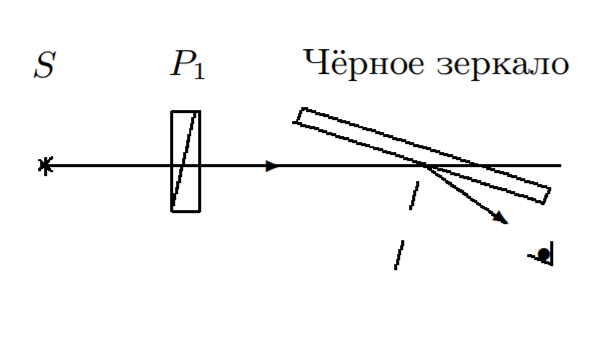
\includegraphics[scale=0.5]{polar_1.png} 
\caption{Определение разрешенного направления поляроида 1}
\label{polar_1}
\end{figure}
Расположим на оптической скамье осветитель S, поляроид $P_1$ и черное зеркало так, как показано на рисунке \ref{polar_1}\\
Поворачивая поляроид вокруг направления луча, а чёрное зеркало вокруг вертикальной оси, методом последовательных приближений добьемся
наименьшей яркости отражённого пятна. Определим разрешённое направление поляроида по лимбу: в нашем случае, это $P_1=52^o$\\
\begin{figure}[h!]
\centering
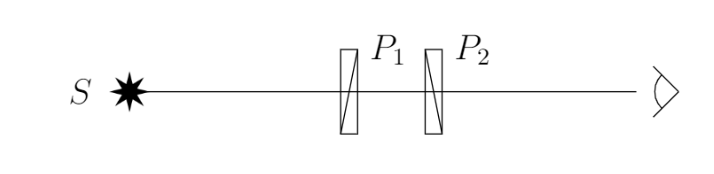
\includegraphics[scale=0.5]{polar_2.png} 
\caption{Определение разрешенного направления поляроида 2}
\label{polar_2}
\end{figure}
Заменив черное зеркало на второй поляроид, получим установку, как на рисунке \ref{polar_2}. Определим разрешенное направление второго поляроида: при скрещивании, если смотреть во 2 поляроид, свет затухнет. $P_2 = 15^o$
\item \textbf{Определение показателя преломления эбонита.}\\
Поставим эбонитовую пластинку перпендикулярно источнику света. Запишем начальный угол $\varphi_0=270$\\
Теперь будем рассматривать свет, отраженный от эбонитовой пластинки. Меняя угол поворота пластинки, добьемся, чтобы интенсивность освещения была минимальна. Тогда мы сможем определить угол Брюстера $\varphi_{\text{Б}} = 215 - 270$ \\
Далее, определим коэффициент отражения $n =tg(\varphi_{\text{Б}})=tg(215-270)\approx 1.43$\\
Сравнивая с табличным значением: $n = 1.6$ Видим, что экспериментальное значение меньше, чем табличное.\\ 
Оценим погрешность в 1$^o$
тогда  $\varphi_{\text{Б}} = 55\pm 1$
\item \textbf{Исследование характера поляризации света в преломлённом и отражённом
от стопы лучах}\\
Соберем установку, состоящую из осветителя и стопы Столетова, которая стоит на месте эбонитового зеркала (рисунок \ref{stopa})
\begin{figure}[h!]
\centering
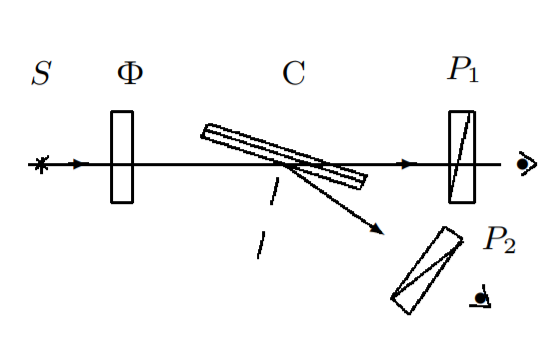
\includegraphics[scale=0.5]{stopa.png} 
\caption{Исследование стопы}
\label{stopa}
\end{figure}
Осветим стопу неполяризованным светом и будем рассматривать ее через поляроиды. \\
В ходе эксперимента, по уже известным засечкам заметим , что при рассмотрении отраженного света, показания поляроида соответствуют значениям для горизонтальной поляризации, а прошедшего -- вертикальной.
\item \textbf{Определение главных направлений двоякопреломляющих пластин}\\
\begin{figure}[h!]
\centering
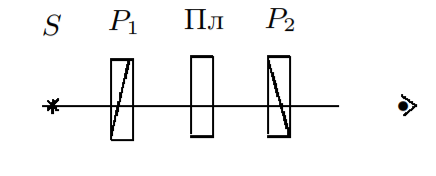
\includegraphics[scale=0.5]{P_0.png} 
\caption{Поиск главных направлений}
\label{P_0}
\end{figure}
Поставим кристаллическую пластинку между двумя скрещенными поляроидами (рисунок \ref{P_0})\\
Вращая пластинку вокруг направления луча, пронаблюдаем за интенсивностью света, проходящего сквозь второй поляроид. Когда яркость проходящего света минимальна, то главное направление пластинки совпадает с направлениями поляроидов.\\
Зафиксируем главные направления.
\item \textbf{Выделение пластин $\lambda/2$ и $\lambda/4$}\\
Добавим к установке \ref{P_0} зеленый фильтр. Установим резрешенное направление поляроида 1 горизонтально, а главные направления исследуемой пластинки под углом $45^o$ к горизонтали. Поляроид 2 будем вращать и наблюдать за характером проходящего через него света.\\
Для пластинки 1 при вращении поляроида яркость освещения практически не изменяется, следовательно, у нее нелинейная поляризация (в нашем случае, эллиптическая), следовательно, это пластинка $\lambda/4$.\\
При вращении поляроида 2 яркость меняется от 0 до какого-то максимума, значит,  поляризация пластинки линейная и это пластинка $\lambda/2$.
\item \textbf{Определение <<быстрой>> и <<медленной>> оси в пластинке $\lambda/4$}\\
\begin{figure}[h!]
\centering
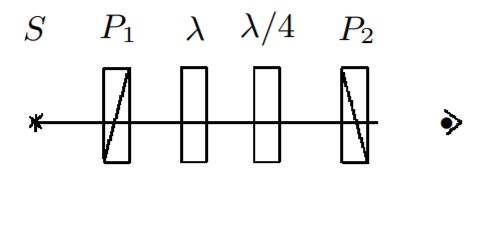
\includegraphics[scale=0.5]{speed.png} 
\caption{Определение направлений большей и меньшей скорости}
\label{speed}
\end{figure}
Поставим между скрещенными поляроидами пластинку чувствительного оттенка, имеющую вид стрелки. Видим, что эта пластинка не меняет поляризацию зеленого света.\\
Уберем зеленый фильтр. Видим, что стрелка имеет пурпурный цвет. Это происходит потому, что зеленый цвет эллиптически не поляризуется, поэтому задерживается поляроидом 2, а красный и фиолетовый являются эллиптически поляризованными и частично проходят через поляроид 2.\\
Добавим к схеме пластинку $\lambda/4$. Получим схему, представленную на рисунке \ref{speed}.
Если у пластинки чувствительного оттенка и пластинки в $\lambda/4$ совпадут главные направления, соответствующие большей скорости
распространения, то разность хода между $E_x$ и $E_y$ для зелёного света составит уже $5\lambda /4$. При освещении
этих пластинок белым светом теперь погасится не зелёная, а более красная
часть спектра, и проходящий свет будет казаться зеленовато-голубым. В этом случае стрелка направлена как на рисунке \ref{5/4}.
\begin{figure}[h!]
\centering
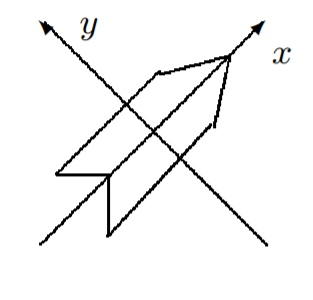
\includegraphics[scale=0.5]{54.png} 
\caption{Пластинка чувствительного оттенка}
\label{5/4}
\end{figure}
Если же главные направления, соответствующие большей скорости распространения, у пластинки чувствительного оттенка и у пластинки
в $\lambda/4$ окажутся перпендикулярными, то проходящий свет приобретёт
оранжево-желтую окраску. Это происходит при направлении стрелки, перпендикулярной рисунку \ref{5/4}
\item   \textbf{Исследование интерференции поляризованных лучей.}\\
Расположим между скрещенными поляроидами мозаичную слюдяную пластинку. При скрещенных поляроидах, картинка будет выглядеть, как: \begin{center}        \begin{tabular}{ |c|c|c|}
		        \hline
		        $3\lambda/4$ зелёный & $\lambda/2$ пурпурный & $3\lambda/4$ зелёный\\
		        \hline
		        $\lambda/4$ красный & - & $\lambda/4$ красный \\
		        \hline
		        $\lambda$ жёлтый & $3\lambda/4$ синий & $\lambda$ жёлтый \\
		        \hline
		        \end{tabular}
\end{center}
Если мы будем вращать пластинку вокруг направления луча, то у нас будет изменяться интенсивность света, но не цвет, в который окрашены пластинки. Это происходит потому, что если поворачивать пластинку, расположенную между
скрещенными поляроидами, то соотношение
амплитуд волн $E_1$ и $E_2$ и разность фаз между ними не изменяются\\
Выставив пластинку под углом $45^o$ вращая поляроид, видим, что интенсивность света остается постоянной, а цвета пластинки изменяются. Это происходит потому, что волны $E_1$ и $E_2$ приобретают дополнительный фазовый сдвиг на $\pi$ для всех спектральных компонент.\\
\end{enumerate}
\paragraph{Выводы:}
\begin{enumerate}
\item Мы определили разрешенные направления поляроидов
\item определили, что отраженный от стопы свет является горизонтально поляризованным, а прошедший -- вертикально
\item оценили угол Брюстера для эбонита, $\varphi_{\text{Б}}=55^o\pm 1^o$. Данные немного расходятся из-за неточно снятых показаний и из-за неидеальности поверхности эбонита
\item Выделили пластинки $\lambda/4$ и $\lambda/2$
\item Определили, что направлению большей скорости соответствует направление вправо, а меньшей -- влево.
\item Исследовали интерференцию поляризованных лучей 
\end{enumerate}
\end{document}